\documentclass[journal=jacsat,manuscript=article]{achemso}
\usepackage[version=3]{mhchem}
\usepackage{amsmath}
\newcommand*\mycommand[1]{\texttt{\emph{#1}}}
\author{James Hamski}
\email{james.hamski@spsmail.cuny.edu}



\title[]{Untappt - Beer Recommendation System}
\makeatletter
\ifxetex
  \usepackage[setpagesize=false, % page size defined by xetex
              unicode=false, % unicode breaks when used with xetex
              xetex]{hyperref}
\else
  \usepackage[unicode=true]{hyperref}
\fi
\hypersetup{breaklinks=true,
            bookmarks=true,
            pdfauthor={},
            pdftitle={},
            colorlinks=true,
            urlcolor=blue,
            linkcolor=magenta,
            pdfborder={0 0 0}}
\urlstyle{same}  % don't use monospace font for urls
\begin{document}
\begin{abstract}
This scenario design uses the Three Question Framework (1) who are your
target users? (2) what are their key goals? (3) how can you help them
accomplish their goals?
\end{abstract}
\section{Introduction}\label{introduction}

Untappt (www.untappt.com) is a web and mobile application that allows
users to search for beers and rate the beer they are drinking. Untappt
as a business appears to rely on:\\
- A subscription service where users can unlock additional functionality
for a subscription. This is known as a `freemium' model.\\
- Advertising: I don't know if Untappt has ads, as I've never seen one
on web or mobile, but the platform could have well-integrated
programmatic advertising.

Both of these business models rely on a loyal user base which frequently
returns to the app.

\section{Identifying target users}\label{identifying-target-users}

I believe the following personas represent target end-users:\\
- ``Beer-nerd'': this is someone who loves beer. They read books and
blogs about beer, travel to breweries on their vacations, know which
local stores have the best selection. They home-brew. When you see them
in any casual setting, they're wearing a brewery tee shirt and they'd
choose death over Bud-lite. They have intense opinions about beer and
the list of beers they've tasted numbers in the hundreds.\\
- ``Bored-with-lite'': this is someone who likes beer well enough, but
they don't know hops from barley and beer is still just a beverage to
them. Maybe they got the impression it was lame to drink a Coors when
that local IPA is available and now it's a habit to go off the beaten
path a bit. They definitely don't like every beer they've ever tried
(what's up with lambics?) and want to remember that nice Pilsner they
had that one time.

\subsection{Identifying the key goals of target end
user}\label{identifying-the-key-goals-of-target-end-user}

\subsubsection{Beer-nerd (BN)}\label{beer-nerd-bn}

The beer nerd (BN) user tries new beers whenever possible. The want a
beer-tracking platform which is up to date, since new breweries and
production runs of beer are created frequently. The beer nerd wants
recommendations that will delight them - obscure, challenging, and
sourced from breweries they may not already know about. The BN users can
be challenged - if you constantly suggest beers that are too similar to
things they've already tried, they may get bored and not return to the
app.\\
\#\#\# Bored-with-lite (BWL)\\
The Bored-with-lite (BWL) user doesn't want to throw good money after
bad when drinking a brew. They know they liked Goose Island IPA once and
they want something a lot like next time the come to Untappt. If a beer
too far afield from their taste is suggested, they may blame the app for
the \$12 beer that they didn't like and not return. If we model beers
and breweries as a graph, BWL users should be shown nearby neighbors to
the beers they've already tried, and suggested results should be
relatively popular varieties.

\subsection{How target end users can accomplish their
goals}\label{how-target-end-users-can-accomplish-their-goals}

Untappt has 4.5 stars on the iTunes App Store with thousands of reviews,
indicating their users are generally satisfied and accomplishing their
goals.

In the mobile app the primary recommendation function is the `Nearby
Beers' page. `Nearby' indicates that the first filter for their
recommendation engine is location. Since brewery distribution is highly
regional, it is important to avoid recommending a beer that is
unavailable in the user's area.

\begin{figure}[htbp]
\centering
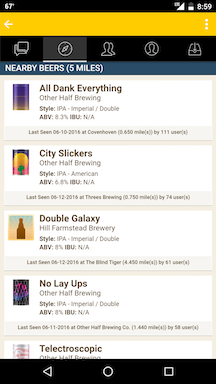
\includegraphics{nearby_beers.png}
\caption{}
\end{figure}

Nearby beers also uses your beer history to suggest brewers and types of
beer similar to those you've rated highly in the past.

To some extent the library of beers in Untappt is crowd-sourced. If you
have a beer but cannot find it in Untappt you can submit it for
inclusion. This relies on BN users to help ensure the app is as current
as possible. Crowd sourcing has drawbacks - it can result in typos,
double-entries, etc. therefore Untappt moderates user-added beers.

\subsection{Reverse engineering
Untappt}\label{reverse-engineering-untappt}

My assessment of the Untappt platform has lead me to believe the
following methods are used in the recommendation engine:\\
1) Geographic filtering by user location 2) Content-based
recommendations - as seen in my screenshot above, most of the
recommended beers come from a NYC brewery that I frequently log in
Untappt called Other Half. I've tried several of their beers and rated
them all high, so now Untappt is suggesting I try some of their newer
brews.

\subsection{Improving Untappt}\label{improving-untappt}

I would improve the Untappt beer recommendations using collaborative
filtering. A collaborative filtering system could match users with beers
based on the likes of users, which have a similar rating history. If
there is a `beer nerd' has a rating vector a short distance from mine,
when that user rates a beer I haven't tried, the platform could
recommend it to me on the guess that our tastes are very similar.

In addition, knowledge based recommendations may be very useful for the
BWL users. Untappt could use basic parameters such as alcohol by volume,
bitterness units, and general popularity of beer types (i.e.~pilsners
over lambics) to improve recommendations for users who have not rated
many beers.

\hypertarget{refs}{}
\end{document}
